


\section{Entity-relationship Model}

StreamFS supports symbolic links, which allows the user to specify non-hierarchical relationships.  Indeed, they can 
be used to express relationships which form a directed graph.  We find that many applications, such as control 
applications and applications that perform aggregation, precede their timeseries queries with multiple queries
to determine indirect relationships between streams.  Fundamentally, the queries were use to ascertain a multiple-hop
relationship between streams and could be easily and efficiently answered with a single graph query.
StreamFS maintains an entity-relationship graph (ERG) that uses the names and symbolic links to construct a queryable 
graph.

The ERG is used throughout our architecture; for answering graph queries by the user and for subscription topic-matching.
The latter is slightly different from the topic-matching mechanism traditionally available in pub-sub systems. 
We discuss the details of our approach in Section~\ref{sec:ProcMngtSchedMain}.


\subsection{ERG to OLAP}
\label{sec:erg2olap}

Many of the operations that users perform are OLAP-style (online analytical processing) operations\cite{Gray1996}. 
OLAP databases build a logical hypercube along multiple dimensions.  The values in the cells are called 
measures.  Queries makes use of the cube to aggregate data along those dimensions.
We provide OLAP-style queries using the ERG.  This is similar to the work proposed by Chen et al.~\cite{Chen2008_olapgraph}.
The time dimension is fixed, the categorical dimension is determined by the hierarchy, and the unit are specified
by the user.

\begin{figure}[h!] %htbp
\centering
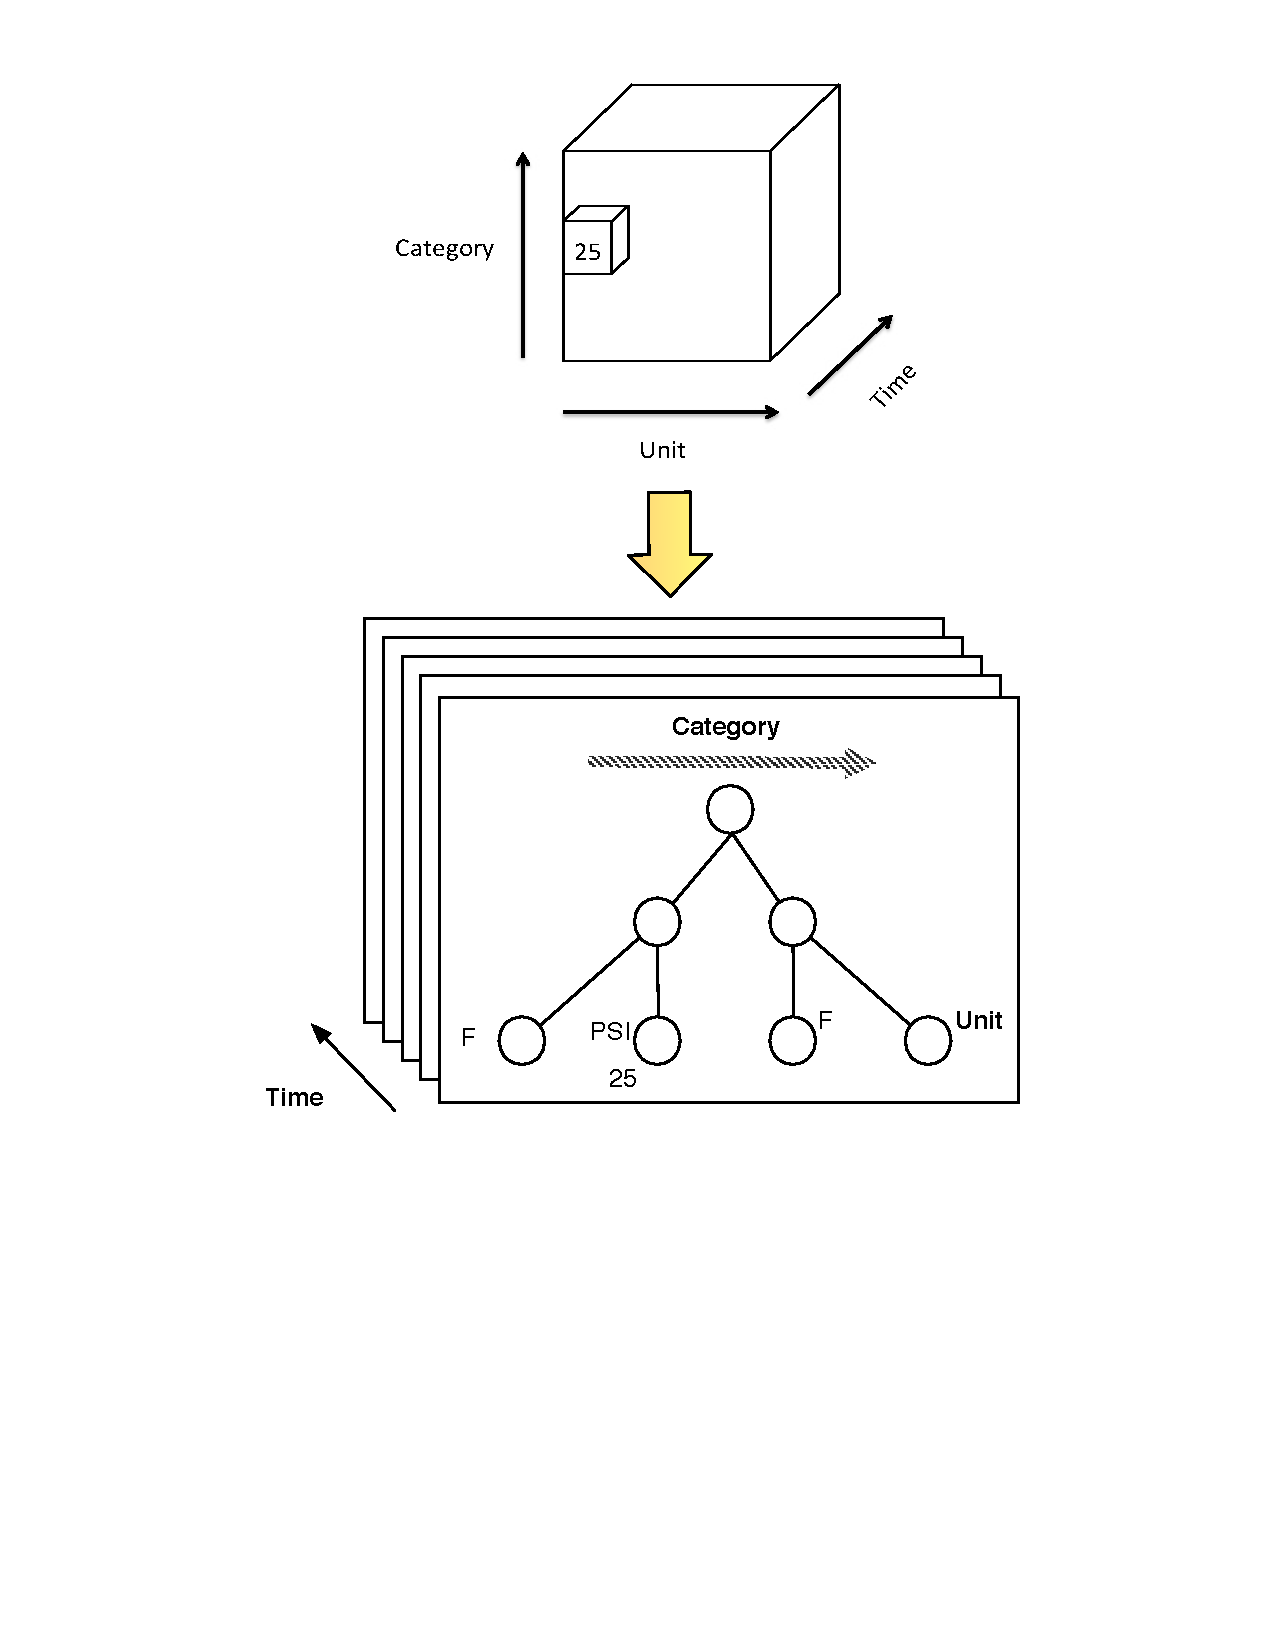
\includegraphics[width=.55\columnwidth]{figs/olaptoerg}
\caption{This figure shows how we translate the OLAP cube to a hierarchical ERG.  Note how the dimensions of the cube translate
to the graph.  The level of the subtree is the category, the unit is specified at the node, and there are values at each node
for every time slice.}
\label{fig:olap2erg}
\end{figure}

% where it can be used more effectively, and how to change the operation of the building -- through better equipment or activity scheduling -- 
% in order to optimize and reduce its energy consumption.
% For building-oriented energy analytics applications the building manager and occupants typically want answers
% to the following set of questions:
Below is a typical list of questions that can be answered efficiently with OLAP-style queries.  

\begin{enumerate}
\item How much energy is consumed in this room/floor/building?  On average?
\item What is the current power draw by this pump? cooling tower? heating sub-system?  Over
		the last month?
% \item How much power is this device currently drawing? Over the last hour?
%\item What percentage of the total building power is being drawn by the plug-load devices? 
% \item How much energy have I consumed today?  Versus yesterday?
\item How much energy does the computing equipment in this building consume?
%\item {\bf For all queries:} What's the trend over time?
\end{enumerate}
\vspace{0.08in}

% Notice, these question span space and time and require aggregation along a dimension, such as power.  
These questions require the ability to answer a series of questions
about energy flow -- energy data aggregated across multiple categories to determine how, where, and the amount used.  
The ability to \emph{slice and dice} the data allows the analyst to gain better insight into how the energy is being used.
Notice how questions translate into categorical and spatio-temporal queries.
There is also a hierarchical grouping characteristic to them.  For example, to answer the first question we must 
aggregate the data from the individual rooms up to the whole building (if the whole building data is not available)
% This hierarchical relationship
% is not as evident in the HVAC sub-components specified in the second question.  However,
% local hierarchically relationships do exist.  For example, 
Also, the cooling system consists of the set of pumps, cooling towers, and condensers in the HVAC system that push condenser
fluid and water to remove heat from spaces in the building.  We can model this as a set of objects and inter-relationships which inform how
to \emph{drill-down}, \emph{roll-up}, and \emph{slice and dice} the data -- traditional OLAP operations.
Figure~\ref{fig:olap2erg} shows how we translate an OLAP cube to a hierarchical arrangement of 
nodes in the ERG.  Time-range queries on any node translates to a slice in the cube along the time dimension.
\emph{Pivoting} along any dimension can be done by taking slices along the ``cube'' in the bottom of that
figure.
% The dynamic aggregation processing model accommodates many common situations where aggregation of feeds is the primary
% objective.  For example, consider a power meter attached to a fan running in a variable air-volume (VAV) unit.
% There can be several hundred VAV units throughout the entire building, one in each space that is controlled by 
% the HVAC system.  An energy auditor may want to determine the energy consumption with respect to either a space 
% or a system or by category.  If these three ``views'' are of interest, there would be three sub-trees in the namespace, 
% rooted at the building: \texttt{/hvac/}\dots\texttt{/vav/fan}, \texttt{/zones/}\dots\texttt{/vav/fan}, 
% and \texttt{/loads/}\dots\texttt{/fans}.  The first is the 
% sub-tree that represents the HVAC sub-components and their inter-connection, the second one describes the set 
% of zones, and the third one is a categorical partitioning of the loads in the building.  With dynamic aggregation,
% as data is received from the each fan stream, it continues up-stream to the aggregation points.
% So, for the total power consumption of the hvac system, you query \texttt{/hvac} (which includes the fans),
% for the total energy consumed in a particular space you query \texttt{/zone/4F/410} for example (which include the fan
% feeding that specific zone), and for a categorical aggregate, you could simple query 
% \texttt{/loads/}\dots\texttt{/fans}.

Unlike a typical OLAP cube, our ``cube'' is dynamic.  As new data comes in, it is immediately used.  Its arrival triggers
the aggregator to interpolate values for all other related streams at that point in time, aggregate them, and update all
the measures in the cube.  We find that many applications that require analytics, typically require OLAP style queries.
% For example, consider the problem of tracking the operational energy consumption of a building.  
We describe how this functionality is useful in performing energy audits and describe its use in
a mobile energy auditing applications presented in Section~\ref{sec:mobileaudit}.



% The main difference between this setup and traditional OLAP is the underlying dynamics of the
% inter-relationships: objects, particularly those meant to represent physical entities, are added and removed and 
% their inter-relationships change over time.  \emph{The natural evolution of buildings and activities 
% within them makes tracking energy-flow fundamentally challenging}.

The entity-relationship model helps simplify these problems, both as an interface to the user and a data structure for the aggregation processes.  
We argue that using the ERG in the building context is reduces the cognitive load and makes the formulation
of such queries easier.  The inter-relationships are explicitly specified and this allows users to 
maintain a structure that is more natural.  Also, it has been shown that a relational model loses this 
information~\cite{SenkoDB}.


% We argue that the 
% use of this model is a cleaner
% fit for this application scenario because it captures important semantic information about the real-world;
% facts critical for picking which questions to ask and how to answer them.  In contrast, it has been shown 
% that a relational model loses this information~\cite{SenkoDB}.

% Lets examine the requirements for answering the first question.
% A building is unware that there are rooms. Typically spaces in a building are called \emph{zones} and, 
% at construction time, walls are added to make rooms within zones.  This makes rooms an abstract
% entity, used to group associated items with respect to it.  It also means
% %The basic control unit for the Heating, Ventilation, and Air conditioning (HVAC) system as well as the electrical 
% %panels and plugs, is a zone, not a room.  
% we typically do not have a single meter that is measuring the energy of a room; it
% must be calculated from the set of energy-consuming constituents.

% What are the energy consuming constituents of a typical room?  It is the set of energy-consumers that
% are active within or onto the room.  Broadly, it consists of three things:

% \begin{itemize}
% \item Plug-loads
% \item Lights
% \item HVAC
% \end{itemize}
% \vspace{0.08in}

% For simplicity of demonstration, lets consider only plug-loads.  In our construction of an entity-relationship
% graph lets assume there are nodes for each plug-load item and each room.  For the room in question, the relationship
% between the plug-loads and the room is child to parent, respectively.  The total energy consumed by
% the plug-loads can be aggregated at the parent node, the room, so the user can query the room for
% the total.  Over time, plug-loads are removed and added to/from the room, but the relationship does not
% change.  This simplifies the query; to obtain the total consumption over time, the query need only
% go to the room node.  The parent-child relationship informs which constituents to aggregate over time
% to calculate the total.

% To realize this design we need to maintain the entity-relationship graph, present it to the user in a meaningful
% way; allowing them to update it directly to capture physical state and relationship changes.  We also need to
% use this graphical structure to direct data flow throughout the underlying network.  This allows us
% to accurately maintain the running aggregates as the deployment and activities churn.

% We present the graph to the user through a filesystem-like naming and linking mechanisms.  The combination of a
% hierarchical naming scheme and support for symbolic links allows the user to access and manipulate underlying objects
% and relationships.  Moreover, the underlying graph structure is overloaded with upstream communication mechanisms
% and buffering to allow data to flow from the data-producing leave nodes to the aggregation-performing
% parent nodes.  Furthermore, the buffering lets us deal with the streaming nature of data flow from the physical
% world to StreamFS and lets us maintain a real-time view of energy flow in the system.
% Traversing the graph provides a natural way for the user to implicitly execute the OLAP operations necessary 
% to give the user the kind of insight into energy usage in the building necessary to understand, optimize and 
% reduce it.

\subsection{Implementation Details}
The graph is maintained in memory.  A typical deployment contains about 10k nodes, so the memory footprint is not that large. 
In our deployments we kept the unit on its own machine with 4 GB of memory.  The footprint is typically several hundred to
about 1 GB in size.  We used a JUNG graph library~\cite{jung} to maintain the graph.

To achieve horizontal scalability, we propose that each ERG unit should be separated into distinct nodes in
a cluster and graph queries should be answered across the cluster.  This is a topic for future work, however, since a typical
building deployment does not require that level of scale.  A collection of buildings, managed through
a single instance of StreamFS, would likely require a clustered implementation of the ERG.















